%\documentclass{article}
\documentclass[border=5pt]{standalone}
\usepackage{tikz}
\usetikzlibrary{decorations.markings}

\tikzset{help lines/.style={very thin,color=gray!50}} % modify the help lines style
\tikzset{->-/.style={decoration={
  markings,
  mark=at position .5 with {\arrow{>}}},postaction={decorate}}}
  
\begin{document}

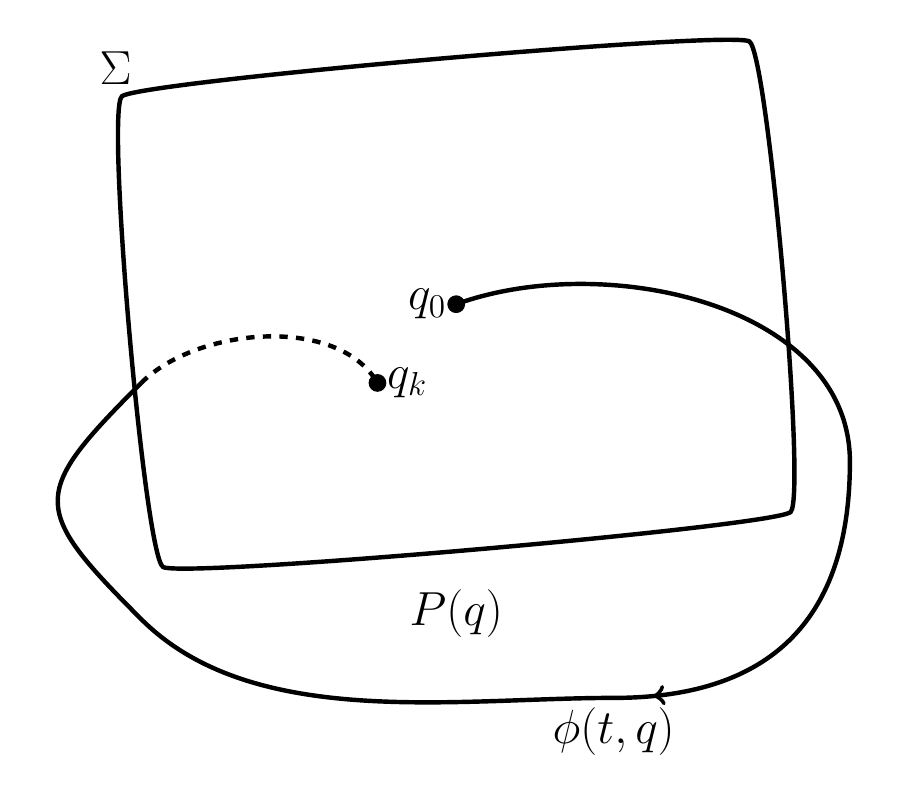
\begin{tikzpicture}[scale=1]
	\coordinate [label=left:\textcolor{black}{\LARGE \(q_0\)}] (x0) at (0,0);
	\coordinate [label=right:\textcolor{black}{\LARGE  \(q_k\)}] (xn) at (-1,-1);
	\coordinate [label=left:\textcolor{black}{\LARGE  \(\Sigma\)}] (sigma) at (-4,3);
	\coordinate [label=below:\textcolor{black}{\LARGE  \(P(q)\)}] (P) at (0,-3.5);
	% define the path of the flow with coordinates
	\coordinate [label=right:\textcolor{blue}{}] (f1) at (5,-2);
	\coordinate [label=below:\textcolor{black}{\LARGE  \(\phi(t,q)\)}] (f2) at (2,-5);
	\coordinate [label=right:\textcolor{blue}{}] (f3) at (-4,-4);
	\coordinate [label=right:\textcolor{blue}{}] (f4) at (-4,-1);
	
%	\draw[help lines] (-10,-10) grid (10,10); %grid
	\filldraw [black] (x0) circle [radius=3pt];
	\filldraw [black] (xn) circle [radius=3pt];

	\draw [ultra thick,black,->-](x0) to[out=20,in=90,distance=2cm] (f1) to[out=-90,in=0,distance=2cm] (f2) to[out=180,in=-45,distance=2cm] (f3) to[out=135,in=-135,distance=2cm] (f4) ;
	\draw [ultra thick, black,dashed] (f4) to[out=45,in=120,distance=1cm] (xn);
	
	\draw [ultra thick] plot [smooth cycle, tension=0.1, rotate=5] coordinates { (-4,-3) (4,-3) (4,3) (-4,3) };


\end{tikzpicture}
\end{document}